\chapter{Projekt architektury oprogramowania}

W tym rozdziale zostanie przedstawiona architektura oprogramowania systemu weryfikacji mówcy w czasie rzeczywistym w przeznaczeniu dla systemów wbudowanych. W pierwszej kolejności zostanie zaprezentowana ogólna struktura zadania weryfikacji mówcy odpowiednio dla fazy modelowania oraz fazy testowania na której to opiera się cały projekt. Następnie zostanie przedstawiony szczegółowy opis zaproponowanej architektury dla aplikacji algorytmów weryfikacji mówcy w czasie rzeczywistym. Dodatkowo zaprezentowana zostania ogólna implementacja rozwiązania problemu dla języka C++ w postaci diagramu UML oraz zostaną omówione struktury i algorytmy sterujące znajdujące się w systemie które są niezależne od wybranych metod z zakresu weryfikacji mówcy. Przykład konkretnego zastosowania omawianej architektury oraz opis implementacji w pełni funkcjonalnego sytemu weryfikacji mówcy znajduje się w kolejnym rozdziale.

\section{Schemat funkcjonalny systemu weryfikacji mówcy.}

W ogólności system weryfikacji mówcy musi sprostać dwóm problemom składającym się na dwa etapy niezależne w czasie: uzyskania modelu mówcy w fazie modelowania (treningu) oraz podjęcie decyzji o weryfikacji mówcy na podstawie wcześniej uzyskanego modelu oraz testowanego sygnału mowy w fazie testowania (weryfikacji). Ponieważ te dwa etapy różnią się na poziomie funkcjonalności zatem struktura wewnętrzna systemów również w pewnym stopniu są różne.

\subsection{Faza modelowania}

Aby system mógł podjąć decyzję o weryfikacji mówcy w jego posiadaniu musi znajdować się wcześniej uzyskany model weryfikowanego mówcy, który wykorzystywany jest do porównania z odpowiednio sparametryzowanym, testowym sygnałem mowy. Odbywa się to w etapie modelowania. Ogólna struktura procesu uzyskiwania modelu mówcy z naciskiem na przepływ danych znajduje się na rysunku (\textbf{\ref{fig:fundiagmodel}}). Zadanie uzyskania modelu mówcy składa się kolejno z etapów:

\begin{figure}[ht!]
  \centering
    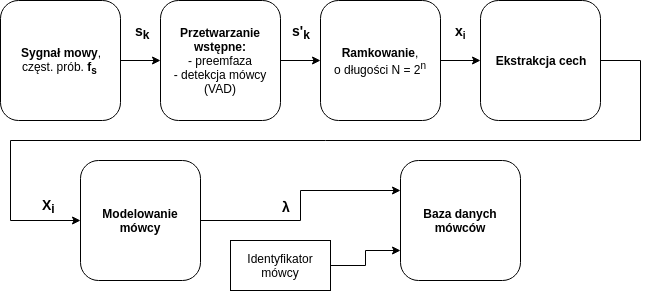
\includegraphics[width=0.9\textwidth]{./fundiagmodel.png}
    \caption{\label{fig:fundiagmodel} Schemat funkcjonalny implementacji systemu weryfikacji mówcy dla etapu modelowania.}
\end{figure}

\begin{enumerate}
\item{\textbf{Akwizycja sygnału mowy}} - wejściem całego sygnału jest spróbkowany z częstotliowścią $f_s$ sygnał mowy $\bm{s_k}$. Dostarczany jest on z bądź to z pamięci komputera jako całość lub dostarczany jest w czasie rzeczywistym jako kolejne próbki. Dla tego drugiego przypadku na ten etap składa się realizacja sprzętowa akwizycji sygnały akustycznego mowy za pomocą przetwornika elektroakustycznego oraz przetwornika analogowo-akustycznego. Ważnym elementem jest również odpowiednie filtrowanie analogowe sygnału - usunięcie składowej stałej oraz filtrowanie częstotliwości wyższych niż połowy częstotliwości próbkowania $f_s$ (filtracja antyaliasingowa).
\item{\textbf{Przetwarzanie wstępne}} - na ten etap mogą składać się wszelkiego rodzaju techniki poprawy jakości sygnału takie jak odszumianie. Najczęściej w systemach weryfikacji mówcy stosuje się tzw. preemfazę - czyli wzmacnianie wyższych częstotliwości sygnału oraz systemy detekcji mówcy (\textit{ang. Voice Activity Detection - VAD})  zwłaszcza dla systemów czasu rzeczywistego. W wyniku przeprowadzonych operacji z sygnału $\bm{s_k}$ otrzymujemy przetworzony sygnał $\bm{s'_k}$.
\item{\textbf{Ramkowanie}} - zwykle w przypadku ekstrakcji cech niskiego poziomu konieczne jest zaaplikowanie ramek na sygnał mowy tak aby uzyskać chwilowe wektory cech. Dla metod ekstrakcji cech wykorzystujących dyskretne przekształcenie Fouriera (DFT) zwykle dobiera się ramki o długościach będących wielokrotnościami dwójki ($N=2^n$). W przypadku takich cech jak LPCC nie jest to warunek konieczny, jednak często stosowany. W wyniku operacji ramkowania otrzymywany jest zbiór wektorów $\bm{x_i}$ o długości N.
\item{\textbf{Ekstrakcja cech}} - na ten etap składa się przetwarzanie ramek sygnału mowy $\bm{x_i}$ na wektory cech oznaczone jako $\bm{X_i}$. Różne techniki wykorzystywane w tym procesie opisano w sekcji \textbf{\ref{featureextraction}}.
\item{\textbf{Modelowanie mówcy}} - w tej części konstruowany jest model mówcy $\bm{\lambda}$ na podstawie zbioru wektorów trenujących $\bm{X_i}$. Różne techniki otrzymywania modeli opisane zostały w sekcji \textbf{\ref{featurematching}}. Model reprezentowany jest najczęściej jako wektor współczynników: w VQ są to centroidy znajdujące się w przestrzeni wektorów, zaś w technice GMM są tą współczynniki wagowe $w_i$ kolejnych funkcji aproksymujących funkcję gęstości prawdopodobieństwa.
\item{\textbf{Zapisanie modelu do bazy danych}} - Wartości parametrów charakteryzujących model mówcy $\bm{\lambda}$ muszą być zapisane na potrzeby fazy weryfikacji. Konieczne jest aby wraz z modelem została zapisana informacja dotycząca tożsamości mówcy - może być to numer identyfikacyjny w postaci danych charakterystycznych dla mówcy. Identyfikator mówcy jest wykorzystywany w fazie weryfikacji razem z modelem.
\end{enumerate}

\subsection{Faza weryfikacji.}

Jeżeli system jest w posiadaniu modelu mówcy za który podaje się mówca od którego testowany sygnał mowy pochodzi, system weryfikacji mówcy może przeprowadzić procedurę weryfikacji. W tym celu musi przedstawić informację identyfikującą weryfikowanego mówcę. Ogólna struktura procesu weryfikacji mówcy z naciskiem na przepływ danych znajduje się na rysunku \textbf{\ref{fig:fundiagverif}}. W omawianej procedurze zachowana jest postać poprzedniego algorytmu aż do momentu uzyskania zbioru wyekstrahowanych cech włącznie. Natomiast zachodzą istotne zmiany co do kolejnych etapów:

\begin{figure}[ht!]
  \centering
    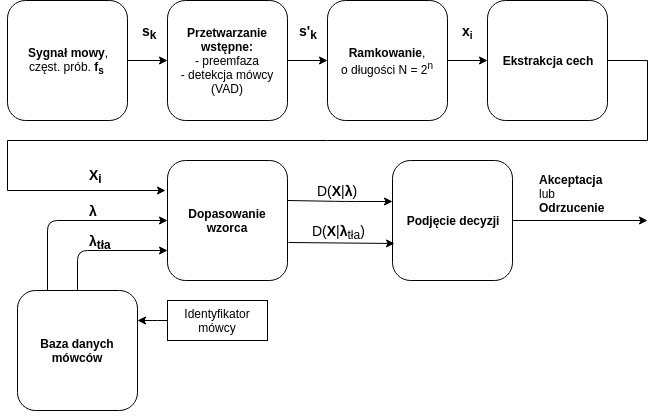
\includegraphics[width=1\textwidth]{./fundiagverif.png}
    \caption{\label{fig:fundiagverif} Schemat funkcjonalny implementacji systemu weryfikacji mówcy dla fazy weryfikacji.}
\end{figure}

\begin{enumerate}
\item{\textbf{Dopasowanie wzorca}} - ten etap korzysta ze zbioru cech $X_i$ w celu weryfikacji mówcy. Podczas tego etapu obliczana jest miara dopasowania pomiędzy wektorami $X_i$ a modelami kolejno $\lambda$ i $\lambda_tła$. W tym przypadku model oznaczony jako $\lambda_tła$ oznacza albo model tła albo model kohorty (w rozumieniu sekcji \textbf{\ref{verif}}). Wyjściem procesu jest wartość liczbowa tej miary dla obu porównań na rysunku oznaczone jako $D(\bm{X}|\bm{\lambda})$ i $D(\bm{X}|\bm{\lambda}_{tla})$. Dla techniki VQ miara dopasowania to wartość funkcji metryki $d(X,C_n)$ gdzie $C-n$ to centroidy modelu. W przypadku techniki GMM miarą dopasowania jest prawdopodobieństwo.
\item{\textbf{Podjęcie decyzji}} - ostatnim etapem razy weryfikacji mówcy jest podjęcie decyzji. Techniki związane z tym zagadnieniem opisano w sekcji \textbf{\ref{verif}}. Decyzja podejmowana jest na podstawie dwóch liczb dostarczonych z poprzedniego bloku: $D(\bm{X}|\bm{\lambda})$ i $D(\bm{X}|\bm{\lambda}_{tla})$ oraz ustalonego przez projektanta progu $\theta$. Wyjściem całego systemu jest zmienna binarna przyjmująca wartości: Akceptacja lub Odrzucenie.
\end{enumerate}

\section{Architektura systemu weryfikacji mówcy dla czasu rzeczywistego}

\begin{figure}[ht!]
  \centering
    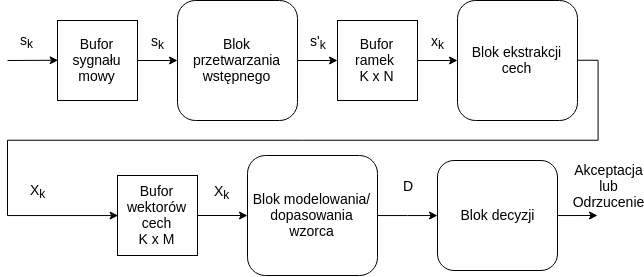
\includegraphics[width=1\textwidth]{./overallrt.png}
    \caption{\label{fig:fundiagverif} Schemat funkcjonalny implementacji systemu weryfikacji mówcy dla fazy weryfikacji.}
\end{figure}
